% !TeX encoding=utf8
% !TeX spellcheck=en-Us
\hyphenation{mea-sur-ements}
\chapter{Setup}
This chapter presents the experimental setup for electroluminescence (EL) measurements. Successful EL measurements consist of charge injection, charge recombination and luminescence detection. Therefore \autoref{sec:GeneralSetup} explaines the general setup. The following \autoref{sec:electricalconnection} explains the Perovskite Cell layout and electrical contacting of the cells. The emitted radiation is detected by a camera with the use of additional optics,  explained in \autoref{sec:luminescencedetection}. The chapter concludes with the consideration of noise and errors.

\section{General Setup}\label{sec:GeneralSetup}
The setup is enclosed in a black housing, shielding the inside from outside light and noise (see \autoref{fig:generalsetup}). All parts inside the chamber are painted black to minimize internal reflections and thereby the detection of stray light. A vacuum pump, voltage source, multimeter and operating table with a computer are connected to the setup from the oustide, providing further utility. Inside the enclosure are the probe holder and camera. To position the camera according to the sample size and used optics, the camera can be moved in three dimensions.
\begin{figure}[h]
	\centering
	\includesvg{Images/ExperimentalSetup/ExperimentalSetupSketch.svg}
	\caption{Schematic of the EL measurement setup. Camera and Probe are positioned inside the setup, and the computer, power supplies and measurement devices are provided from the outside. Two multimeters are used to measure the voltage drop and current sourced.}
	\label{fig:generalsetup}
\end{figure}
\FloatBarrier
\section{Electrical Connection}\label{sec:electricalconnection}
Perovskite Solar Cells (PSCs) are manufactured on 25 mm x25 mm glass substrates (see \autoref{fig:perolayouttop}). Four cells are deposited on one substrate, each single cell having dimensions of 4 mm x 3.5 mm. The cell stack consists of a glass substrate, with a xyz nm thick layer of Indium Tin Oxide (short ITO) deposited ontop. xyz nm of Spiro-TTB are used as a Hole Transport Layer (HTL), followed by 500 nm of methylammonium lead triiodide (short MAPI) as the absorbing layer. The top side of the MAPI is contacted with xyz nm of C60 and BCP, acting as the Electron Transport Layer (short ETL). In the end of the fabrication process, xyz nm Gold are deposited on top of the ITO and the C60/BCP. To succesfully contact the PSC a holder with four pins is used. The holder uses two pins to check proper contacting of the PSC and the other two to source voltage.
\begin{figure}
	\centering
	\includesvg{Images/ExperimentalSetup/Pero_Layout_side}
	\caption{Schematic layout of the perovskite solar cell. Not to scale.}
	\label{fig:perolayouttop}
\end{figure}

The holder is electrically connected to a power supply\footnote{Kukusuki}, in series with a 100 m$\Omega$ resistance, R, and two multimeters\footnote{Keithley 2000 Multimeter} (see \autoref{fig:generalsetup}). The multimeter measures the voltage drop across the PSC. The other multimeter measures the voltage drop across the resistor and the flowing current I is then calculated by Ohm's law:
\begin{equation}
	I = \frac{U}{R}.
\end{equation}

Structured wells with a vacuum connection fixate the PSC on the holder. This ensures mechanical and electrical contact stability throughout the measurement.

This setup enables safe contacting of the probes inside the enclosure. After correct poling, charges are injected and recombine. The emitted radiation is detected by a camera, what requires the usage of filters and optics.

\section{Luminescence detection}\label{sec:luminescencedetection}
In the setup a ccd camera detects the emitted luminescence. The camera detects radiation over a wide range of wavelengths, while the perovskite emits luminescence only at specific wavelengths with small halbwertsbreite. Therefore filters are used to detect only the EL radiation. Optics focus the emitted radiation at a specific distance onto the imaging sensor. This chapter explains the used components and physical processes.
\subsection{Filters}
Between probe and sensor a filter\footnote{bk-Interferenzoptik, custom made product} is used to filter the wavelengths reaching the detector. In filters absorption or interference are used to either transmit or reflect specific wavelengths. The filter in the setup is a bandpass filter and chosen accordingly to the luminescence emission spectrum of the PSC (see \autoref{fig:spectrum_perofilter}). This reduces the detected wavelengths to 780 nm to 800 nm, the interval with maximal intensity of the PSC, which enables maximum sensitivity to the emitted radiation and limits the detection of stray light. %This filter is sensitive to high intensity, ... , which is above/below the luminescence emission of the PSC. 

\begin{figure}[h]
	\centering
	\includesvg{Images/ExperimentalSetup/SpectralEL/PL_spectrum_MAPIcell_with_filter_PPT.svg}
	\caption{Emitted luminescence spectrum of the perovskite and transmission function of the filter. Taken from 2015 Predicting Voc. DIESES BILD DURCH PL MESSUNG VON MARVIN ERSETZEN ODER SO AUS INSTITUT!}
	\label{fig:spectrum_perofilter}
\end{figure}
\subsection{Optics}
Optics focus the radiation onto a charge coupled sensor (CCD). This setup uses a lens\footnote{Pentax, C2514-M (KP)} with a focus length of 25 mm and an aperature of 1.4, as listed by the manufacturer. The lens is positioned at the minimal object distance of  25 cm away from the PSC and mounted directly to the camera with a C-mount.
\\
SKETCH FOR LENS SYSTEM
\\


\subsection{Charge Coupled Detectors}
The radiation is focused onto a charge coupled detector (CCD) sensor\footnote{Sony ICX285-AL} in a camera\footnote{PCO, sensicam qe}. CCD sensors are silicon chips structured into small squares, called wells \cite{SchnellCCD1993}(see \autoref{fig:ccdsensor}). The number of wells correspond to the number of pixel in the taken picture. Radiation generates charges, electrons and holes, and externally applied voltages seperate and trap the charges in the wells. For a specific time, called exposure time, radiation hits the sensor and charges accumulate in the wells. The amount of generated electrons per incoming photon is called the quantum efficiency (QE), and depends on the sensor material and energy of the photon. The QE for the chosen sensor peaks at 500 nm and decays for larger wavelengths (compare \autoref{fig:pcosensicamqe}). For the wavelengths transmitted by the filter (see section before), the QE deops to about 10 \%, which reduces the sensitivity. After the exposure time a series of voltages is applied to shift the charges from the light sensitive wells to opaque covered wells. Then the charges are extracted row by row and the voltage of each well is measured. An A/D converter convertes the voltage into an digital signal, which is saved and later processed.
\begin{figure}
	\centering
	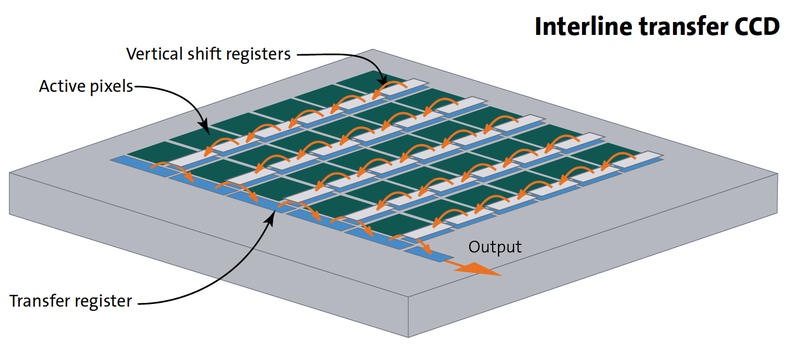
\includegraphics[width=\linewidth]{Images/ExperimentalSetup/ccd-sensor-interline-transfer-en}
	\caption{Schematic represantation of a CCD sensor. Radiation generates charges in the active pixels and is transferred through vertical shift registers to the transfer register. Taken from \cite{StemmerCCD}.}
	\label{fig:ccdsensor}
\end{figure}

This process measures the EL distribution over the PSC surface. However several sources of errors occur, which are discussed in the next section.
%\begin{figure}
%	\centering
%	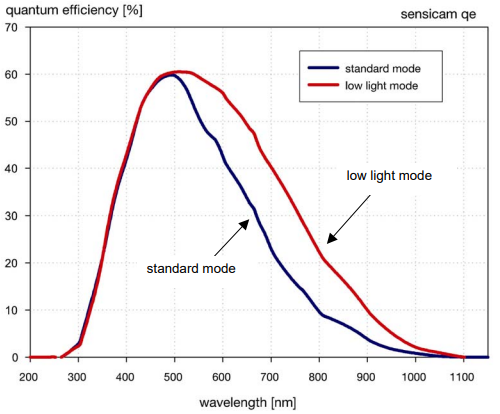
\includegraphics[width=\linewidth]{Images/ExperimentalSetup/PCO_sensicam_QE}
%	\caption{Quantum efficiency of the PCO sensicam qe, given by the manufacturer.}
%	\label{fig:pcosensicamqe}
%\end{figure}

\section{Noise and measurement errors}
Several sources of errors deviate the measured signal from the physical value. Common errors are dark noise, readout noise and hot or cold pixel. Dark noise refers to the thermal generation of electrons, depending on the temperature and the material's properties. To reduce thermal generation the CCD sensor is cooled to -12 C. To further reduce dark noise, Images without illumination or applied voltage are taken, and subtracted from the EL image.\\

Other sources of errors happen when the electrons are shifted from well to well, called readout noise. The manufactur specifies the read out noise of 5 electrons. This relates to about one count, with an analog to digital conversion efficiency of 4 electrons per count.\cite{ManualSensicam}
 